\section{Data inventory and qualitative examples}
\label{app:data}
The inventory of consumer images contains 40,587 records, matching the sum of the four partition counts in Table~\ref{tab:data}, whereas 40,550 successful crops are reported. Split generation filters \texttt{crops.csv} to successful detections before assigning partitions and writes \texttt{manifest.csv} and \texttt{summary.json}, but these generated files are absent from the available checkout. Consequently, the available records do not establish whether the discrepancy reflects different preprocessing revisions, and the partition counts remain reported values pending reconciliation with the manifest for the run and crop log.

The MEDISEG inventory similarly distinguishes 14,069 annotated instances from 13,973 evaluated queries. The source paper reports 8,262 images~\citep{chu2026mediseg}, whereas the local retained set contains 8,261. Download and preprocessing records are described in \texttt{epills/docs/datasets.md}. Representative views of the same identity are shown in the main text, Figure~\ref{fig:examples}.


\begin{figure}[!htbp]
  \centering
  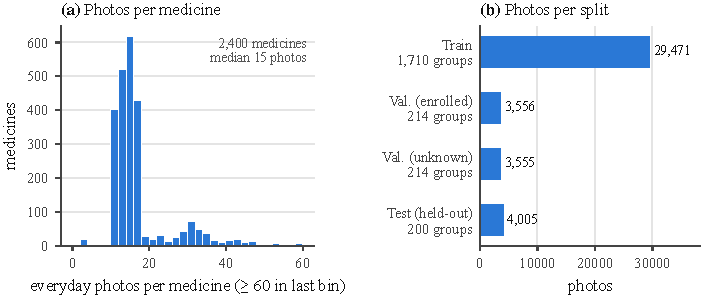
\includegraphics[width=0.94\linewidth,height=0.25\textheight,keepaspectratio]{fig03_data_statistics.pdf}
  \caption{Statistics for C3PI consumer images reproduced from the supplied project materials. (a) Reported images per pill type, defined by NDC9 and product part, with counts of 60 or more pooled in the final bin. (b) Reported partition sizes and counts of appearance groups. Types sharing recorded imprint, shape, colour and size are assigned to the same group, and each group is assigned to one partition. Groups containing an ePillID fold-4 holdout identity form the held-out test partition. The image counts total 40,587 and remain unreconciled with the reported 40,550 successful crops.}
  \label{fig:data-statistics}
\end{figure}

\FloatBarrier
\section{Architecture and training configuration}
\label{app:configuration}
The main training schedule and augmentation are specified in Section~\ref{sec:training}. Table~\ref{tab:arch} lists the layer configuration during inference. Layers after the pretrained backbones use Glorot-uniform initialisation.

\begin{table}[!htbp]
  \caption{The network's layers (inference mode). Pretrained weights: VGG16 on ImageNet, ViT-B/16 on ImageNet-21k.}
  \label{tab:arch}
  \centering
  \small
  \begin{tabular}{@{}p{0.19\linewidth}p{0.62\linewidth}r@{}}
    \toprule
    Block & Details & Output \\
    \midrule
    CNN branch & VGG16 conv.\ blocks $\to$ CBAM $\to$ global average pool $\to$ Dense, ReLU & 256 \\
    ViT branch & ViT-B/16 (\texttt{vit-base-patch16-224-in21k}), pooler output & 768 \\
    Capsule fusion & per branch: Dense 256, ReLU, dropout 0.4, Dense 256, batch norm; dynamic routing, 2 iterations,
      residual update & 256 \\
    Refinement & 4 tokens $\times$ 64 + learned positions; 2 post-norm encoder layers (4 heads, feed-forward width 128, dropout
      0.4); mean pool & 64 \\
    Embedding head & Linear, $\ell_2$ normalisation & 256 \\
    Auxiliary heads & shape (softmax), colour (multi-label sigmoid) & -- \\
    \bottomrule
  \end{tabular}
\end{table}

\FloatBarrier
\section{Calibration and training diagnostics}
\label{app:calibration}
The main evaluation uses rejection, ambiguity and imprint re-ranking parameters selected on validation data. Calibration curves, sequential training changes and training trajectories are collected here to distinguish the selection procedure from the held-out results.

The project plan defines validation targets for a gallery of ten medicines enrolled from three photographs per medicine (Table~\ref{tab:targets}). These are development criteria, not held-out performance claims. In particular, top-1 within the gallery, correct naming at a rejection operating point, and acceptance of foreign queries are distinct measures. Held-out results are reported separately in Table~\ref{tab:main}.

\begin{table}[!htbp]
\centering\small
\caption{Validation targets from the project plan and reported measurements for run 4. These measurements concern validation galleries, with held-out results reported separately.}
\label{tab:targets}
\begin{tabular}{@{}lrr@{}}
\toprule
Measure & Target & Run 4 \\
\midrule
Top-1 within the gallery & $\ge95\%$ & 97.9\% \\
Own-versus-foreign AUROC & $\ge0.90$ & 0.978 \\
Correct naming at 95\% foreign rejection & $\ge80\%$ & 87.9\% \\
Misidentification rate among enrolled queries & $\le 2\%$ & 1.2\% \\
\bottomrule
\end{tabular}
\end{table}

\begin{figure}[!htbp]
  \centering
  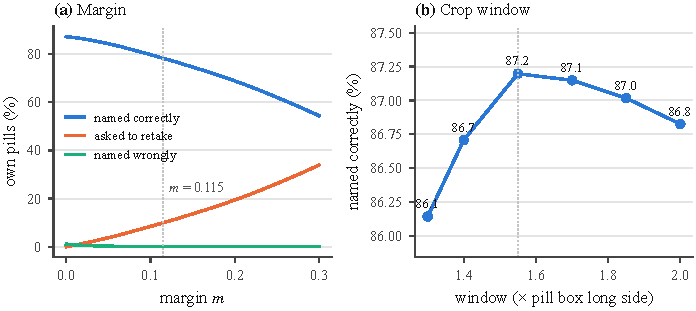
\includegraphics[width=0.92\linewidth,height=0.23\textheight,keepaspectratio]{fig06_calibration.pdf}
  \caption{Settings chosen on validation (1,000 simulated patients, 10 medicines, 3 enrolment photos; $\tau$ rejects
    95\% of other medicines). (a) The margin trades correct names for retakes while wrong names stay near zero.
    (b) Correct naming across crop windows, shown with a narrow $y$-range.}
  \label{fig:calib}
\end{figure}

\begin{table}[!htbp]
  \caption{Sequential design comparisons and parameter sweeps. Multiple changes are combined between runs, so these comparisons do not isolate individual components. Validation results are shown unless a held-out comparison is referenced.}
  \label{tab:ablation}
  \centering
  \small
  \begin{tabular}{@{}p{0.34\linewidth}p{0.46\linewidth}p{0.12\linewidth}@{}}
    \toprule
    Change & Effect & Kept \\
    \midrule
    Run 1$\to$2: lower LRs ($3{\times}10^{-5}$, $10^{-5}$), separate ArcFace LR, margin warm-up & top-1 in 10
      medicines 77.2$\to$98.3\%; AUROC 0.78$\to$0.981; correct at 95\% rejection 17$\to$90.7\%; dims
      $\approx$3$\to$12--15 & yes \\
    Run 2$\to$3: + studio reference photos & validation 98.1\%; higher strict ePillID MAP@1 (Table~\ref{tab:main}) & yes \\
    Run 3$\to$4: + photo and augmentation with crop jitter & higher MEDISEG accuracy with lower C3PI accuracy (Table~\ref{tab:main})
      & yes \\
    Crop window 1.3--2.0$\times$ & named correctly 86.1--87.2\% & 1.55 \\
    Margin $m$ 0--0.3 & named correctly 87$\to$54\%; retakes 0$\to$34\% & 0.115 \\
    Imprint re-ranking $\alpha$, $K$ & top-1 72.1\% ($\alpha{=}0$)$\to$81.6\%; \emph{test} 71.6$\to$80.2\%
      & 0.05, 100 \\
    Gallery check: distinct tokens only & named wrongly 35$\to$30; other pills accepted 6,158$\to$6,150 & yes \\
    Official ePillID protocol (runs 5--7) & ePillID MAP 0.57--0.60; MEDISEG 52--54\% & benchmark \\
    \bottomrule
  \end{tabular}
\end{table}

\begin{figure}[!htbp]
  \centering
  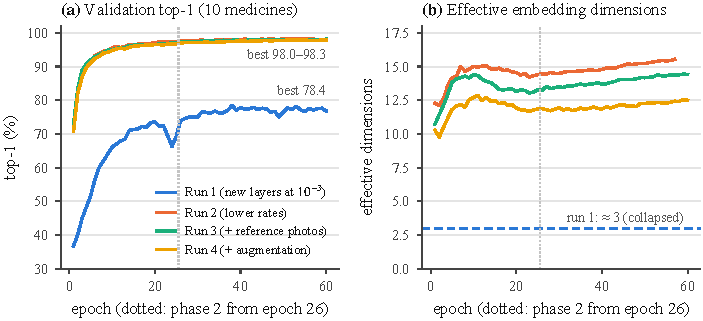
\includegraphics[width=0.92\linewidth,height=0.23\textheight,keepaspectratio]{fig05_training_curves.pdf}
  \caption{Training. (a) Validation top-1 within a gallery of 10 medicines never trained on. (b) Effective embedding
    dimensions: with the new layers at $10^{-3}$ the embedding collapsed to about 3.}
  \label{fig:training}
\end{figure}
\FloatBarrier
\section{Additional error analysis}
\label{app:errors}
\label{sec:errors}

\paragraph{Stratified analysis of imprint reading.} Figure~\ref{fig:imprint} reports validation recovery by recorded imprint type, rater visibility, size and shape. The source analysis uses 7,068 photographs of medicines with a recorded imprint. The corresponding interpretation is given in Section~\ref{sec:error-analysis}.

\begin{figure}[!htbp]
  \centering
  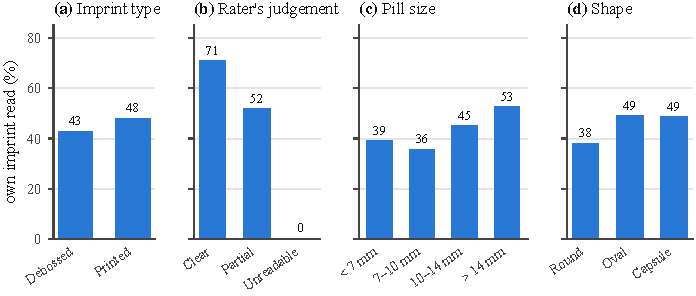
\includegraphics[width=0.92\linewidth,height=0.23\textheight,keepaspectratio]{fig11_imprint_reading.pdf}
  \caption{Share of validation photos on which a token of the pill's own imprint is read (Florence-2-large, zero-shot),
    by imprint type, C3PI rater's judgement of visibility, pill size and shape.}
  \label{fig:imprint}
\end{figure}

\paragraph{Look-alike stress tests.} Both members of each pair are enrolled in the same gallery. Figure~\ref{fig:lookalike} compares matching by appearance alone with the imprint check for different strengths of the same ingredient and pairs from the same manufacturer. The latter share imprint prefixes, including Teva's `TV'. Overall confusion for pairs from the same manufacturer is 0.01\%, but the aggregate masks errors concentrated in individual pairs discussed in Section~\ref{sec:error-analysis}.

\begin{figure}[!htbp]
  \centering
  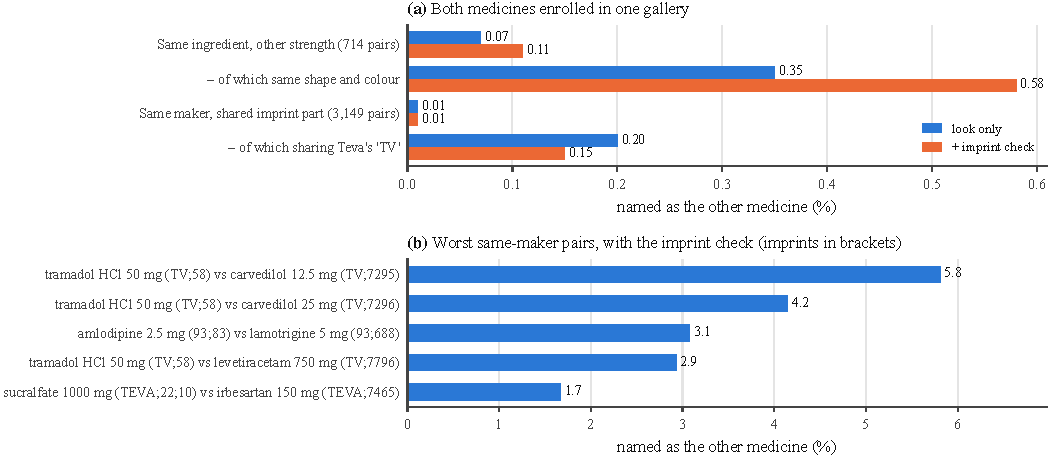
\includegraphics[width=0.92\linewidth,height=0.23\textheight,keepaspectratio]{fig16_lookalike_error_analysis.pdf}
  \caption{Look-alikes, with both medicines enrolled in one gallery. (a) Rates of wrong naming by kind of pair, look only
    and with the imprint check. (b) The worst pairs from the same manufacturer.}
  \label{fig:lookalike}
\end{figure}

\paragraph{Representation diagnostics.} Tracing individual queries yields capsule routing weights of approximately 9\% for the CNN and 91\% for the ViT. Attention between refinement tokens is nearly uniform, describing the feature use observed for these queries. The independent contributions of the branches and fusion mechanism remain unresolved because controlled architectural ablations were not performed.

\paragraph{Rejected variants.} Table~\ref{tab:negative} retains the results of reader adaptation and other rejected variants. Its gallery entries for wrong naming are counts within their respective evaluation configurations, rather than the pooled percentages reported for held-out galleries in Table~\ref{tab:main}.

\begin{table}[!htbp]
  \caption{What did not work (validation).}
  \label{tab:negative}
  \centering
  \small
  \begin{tabular}{@{}p{0.34\linewidth}p{0.46\linewidth}p{0.12\linewidth}@{}}
    \toprule
    Tried & Result & Decision \\
    \midrule
    LoRA of Florence-2-large, v1 (19,312 photos of training medicines) & imprints read 44.0$\to$53.5\%, but
      memorised imprints written onto new pills; identification and gallery check worse & rejected \\
    LoRA v2 (also learns to output nothing on unreadable photos) & own imprint read 45.0$\to$50.7\%; identification
      82.0$\to$83.0\%; gallery wrong names 30$\to$61 & rejected \\
    Look-alike characters (O/0, B/8) treated as equal & measured and dropped & rejected \\
    Scoring each candidate's imprint separately & measured and dropped & rejected \\
    Runs 6--7: stronger fine-tuning; training aligned with the benchmark & better validation and MEDISEG, not ePillID & not
      served \\
    \bottomrule
  \end{tabular}
\end{table}

\FloatBarrier
\section{Implementation and project resources}
\label{app:development}
\label{sec:impl}

The implementation environment reported in the project materials is Python 3.13.15, PyTorch 2.11.0 with CUDA 12.8, and Hugging Face Transformers 5.19.0. Training uses one NVIDIA RTX 4080 SUPER with 16\,GB memory. The pipeline exposes separate stages for partitioning, training, gallery calibration, held-out evaluation, catalogue re-ranking and confidence calibration. The corresponding scripts write configuration, calibration and evaluation records to the run directory.

With the project environment activated, the following PowerShell commands are run from \texttt{epills/}. They reproduce the documented sequence when the required datasets, reference catalogue and cached OCR outputs have been prepared as described in the repository. 

\begin{quote}\small
\begin{verbatim}
$run = 'outputs/runs/stage2_run4'
python scripts/make_splits.py
python scripts/train_stage2.py --config configs/stage2_run4.yaml
python scripts/calibrate_stage2.py --run $run `
  --windows 1.3 1.4 1.55 1.7 1.85 2.0
python scripts/evaluate_stage2.py --run $run
python scripts/tune_identify_rerank.py --run $run --ocr large_c92
python scripts/evaluate_identify_topk.py --run $run --ocr large_c92
python scripts/calibrate_identify.py --run $run --ocr large_c92
python scripts/make_paper_figures.py
\end{verbatim}
\end{quote}

\subsection{Project resources and application prototype}
\label{app:resources}
The image model is deployed through the Hugging Face interface listed in Table~\ref{tab:resources}. A separate care agent application is being developed around this model service, with its deployment and source maintained independently. Its deployment demonstrates application integration in progress. The recognition results in this report evaluate the image pipeline, rather than the agent's medication management behaviour.

\begin{table}[!htbp]
\centering\small
\caption{Project resources supplied by the authors. The care agent application remains under development, and these deployment links document the available demonstrations.}
\label{tab:resources}
\begin{tabular}{@{}p{0.22\linewidth}p{0.73\linewidth}@{}}
\toprule
Resource & Link \\
\midrule
Model demo & \url{https://davidpansx-pharmascan-api.hf.space/ui/} \\
Model source & \url{https://github.com/398-21/ultrasound_Model} \\
Care agent demo & \url{https://medithread.vercel.app} \\
Care agent source & \url{https://github.com/SpectateurLinlan/pharmascan-care-agent} \\
\bottomrule
\end{tabular}
\end{table}

\subsection{Source attribution and report preparation}
The model implementation uses PyTorch and Hugging Face Transformers\footnote{\url{https://github.com/huggingface/transformers}}, with reused project and benchmark code identified in Section~\ref{sec:approach}. The research-paper-writing skill was used for language polishing.
